\documentclass[conference]{IEEEtran}
\IEEEoverridecommandlockouts
\usepackage{cite}
\usepackage{amsmath,amssymb,amsfonts}
\usepackage{graphicx}
\usepackage{booktabs}
\usepackage{multirow}
\usepackage{xcolor}
\usepackage[hidelinks]{hyperref}
\usepackage{url}
\usepackage{algorithm}
\usepackage{algorithmic}
\def\BibTeX{{\rm B\kern-.05em{\sc i\kern-.025em b}\kern-.08em T\kern-.1667em\lower.7ex\hbox{E}\kern-.125emX}}
\newcommand{\selfcal}{\textsc{SelfCal}}
\newcommand{\selftrig}{\textsc{SelfTrig}}
\newcommand{\chat}{\hat{c}}

\begin{document}

\title{Do Conformal Guarantees Expire?\\Label-Free Recalibration of Prediction Sets on a Decade-Long Stream of Scientific Abstracts}

\author{\IEEEauthorblockN{Jeremiah Joseph}
\IEEEauthorblockA{\textit{Apex High School}\\
Apex, North Carolina, USA\\
jeremiahdjoseph843@gmail.com}}

\maketitle

\begin{abstract}
Conformal prediction turns any classifier into a set-valued predictor with a finite-sample coverage guarantee, but the guarantee assumes the calibration data and future data are exchangeable. Real data streams are not. We study how far and how fast this guarantee erodes on a large, naturally drifting stream: 98{,}082 arXiv computer-science abstracts sampled uniformly over 164 consecutive months (2013--2026) and classified into 12 categories with a frozen sentence-embedding classifier. A threshold calibrated once on 2018 holds its nominal 90\% coverage for roughly four years and then decays to 82.5\% in 2026; class-conditional (Mondrian) calibration does not help, showing that the loss is driven by within-category content drift rather than by shifting category proportions. We then observe that the classifier's \emph{own} probabilities, after temperature scaling on the calibration year, yield a label-free monthly estimate of coverage that tracks the true value with a mean absolute error of 0.014. This motivates two simple mechanisms that need no new labels: \selfcal{} re-selects the conformal threshold every month from unlabeled inputs so that the estimated coverage hits the target, and \selftrig{} requests labels only when the estimate falls below the target. On the 92-month test stream, \selfcal{} restores mean coverage to 0.898 with no month below 0.85, matching a sliding-window recalibration that consumes every label, and \selftrig{} reaches 0.890 while labeling only 3.3\% of months. Results replicate on a second deployment window, a lexical TF-IDF model, and a 95\% target. Code and data-processing scripts are released.
\end{abstract}

\begin{IEEEkeywords}
conformal prediction, distribution shift, concept drift, data streams, uncertainty quantification, scientific literature
\end{IEEEkeywords}

\section{Introduction}
Systems that route, tag, or recommend documents at scale increasingly need calibrated uncertainty, not only a top-1 label. Conformal prediction (CP)~\cite{vovk2005algorithmic,angelopoulos2023gentle} offers an attractive answer: wrap \emph{any} classifier and output a set of labels that contains the true label with probability at least $1-\alpha$. The guarantee is distribution-free and holds with finite samples, which is why it has spread quickly into recommender systems~\cite{wang2025confidence}, clinical time series, and LLM pipelines. Its one assumption is that calibration and test points are exchangeable.

Data streams violate this assumption slowly and silently. The vocabulary of a field changes, new sub-topics appear, and category proportions shift. A classifier trained and calibrated once is typically kept frozen in production because retraining is expensive, but nothing in the CP machinery warns the operator that the ``90\%'' printed on the dashboard is no longer true. Adaptive methods exist~\cite{gibbs2021adaptive,barber2023beyond,zaffran2022adaptive}, yet all of them consume fresh \emph{labels} at every step. In many deployments labels arrive late, cost money, or never arrive.

This paper asks two questions on a stream that is large, public, and drifts for natural reasons: \emph{(i) how quickly does a conformal guarantee expire, and (ii) can it be maintained without labels?} We use arXiv, the same stream that motivates recent work on topic discovery~\cite{li2025scitopic} and fresh-vector search~\cite{lai2025updatable}, and make the following contributions.
\begin{itemize}
\item \textbf{A longitudinal measurement.} We track split-conformal coverage month by month for eight years after calibration on 98k abstracts. Coverage decays from 0.89 to 0.82, the decay accelerates sharply after 2023, and Mondrian (class-conditional) calibration does not prevent it (Sec.~\ref{sec:expiry}).
\item \textbf{A label-free coverage monitor.} We show that the expected coverage implied by the classifier's temperature-scaled probabilities, corrected by a single offset learned on the calibration year, tracks the true coverage of the drifting stream (Pearson $r{=}0.82$, MAE 0.014) (Sec.~\ref{sec:estimator}).
\item \textbf{Two label-free mechanisms.} \selfcal{} recalibrates the threshold from unlabeled inputs; \selftrig{} spends a label budget only when the monitor says so. With zero labels \selfcal{} matches a fully-labeled sliding window (0.898 vs.\ 0.899 mean coverage, no month below 0.85); \selftrig{} matches periodic recalibration while requesting 20--40\% as many labels (Sec.~\ref{sec:results}).
\item \textbf{Replication.} Findings hold for a second deployment window, a lexical TF-IDF classifier, and $\alpha{=}0.05$; we also report an honest failure mode (miscalibrated probabilities) and its fix.
\end{itemize}

\section{Background and Related Work}
\textbf{Split conformal classification.} Let $\hat p(x)\in\Delta^{K}$ be a classifier's probability vector. With the least-ambiguous-set score $s(x,y)=1-\hat p_y(x)$~\cite{sadinle2019least}, split CP computes scores on $n$ held-out calibration pairs, takes $q=$ the $\lceil (n{+}1)(1{-}\alpha)\rceil/n$ empirical quantile, and predicts $C(x)=\{k: 1-\hat p_k(x)\le q\}$. If calibration and test points are exchangeable, $\Pr(Y\in C(X))\ge 1-\alpha$~\cite{vovk2005algorithmic}. Other scores (e.g., APS~\cite{romano2020classification}) trade set size for adaptivity; our method is score-agnostic and we use LAC for its small sets.

\textbf{CP under shift.} Weighted CP reweights calibration scores by a likelihood ratio~\cite{tibshirani2019covariate} or, beyond exchangeability, by fixed weights such as time decay with a coverage bound that degrades gracefully with the total variation between distributions~\cite{barber2023beyond}. Adaptive conformal inference (ACI) treats $\alpha$ as an online parameter updated by the observed miscoverage~\cite{gibbs2021adaptive}, with later refinements~\cite{zaffran2022adaptive,bhatnagar2023improved}. All of these require the label of each (or of a recent window of) test points. We use them as label-rich upper bounds.

\textbf{Drift detection.} Concept-drift adaptation is a mature field~\cite{gama2014survey,lu2019learning}. Black-box shift detection monitors the \emph{outputs} of a fixed classifier~\cite{lipton2018detecting,rabanser2019failing}, and average-confidence or thresholded-confidence statistics can predict a classifier's \emph{accuracy} on unlabeled shifted data~\cite{guillory2021predicting,garg2022leveraging}. Our monitor is in this spirit but tracks a quantity that is directly actionable for CP: the model-implied coverage of its own prediction sets, which we then use to reselect the threshold. We are not aware of prior work that uses it to recalibrate conformal thresholds without labels, nor of a multi-year longitudinal measurement of conformal coverage on a natural text stream.

\section{Method}
\subsection{Setting}
A classifier $\hat p$ is trained once and frozen. Labeled calibration data $\mathcal{D}_0$ come from one period (a \emph{calibration year}). Afterwards the stream arrives in monthly batches $\mathcal{B}_1,\mathcal{B}_2,\dots$ of inputs; the operator must emit $C(x)$ for every $x\in\mathcal{B}_t$ \emph{before} any label of $\mathcal{B}_t$ can be seen, and may pay to obtain the labels of a batch after it has been served. We measure (a) empirical monthly coverage $\bar{c}_t$ and set size, and (b) the fraction of months whose labels were requested (the \emph{label budget}).

\subsection{A label-free coverage estimate}\label{sec:method-est}
Fix a threshold $q$ and let $C_q(x)=\{k:1-\hat p_k(x)\le q\}$. If $\hat p$ were exactly calibrated, i.e.\ $\Pr(Y{=}k\mid X{=}x)=\hat p_k(x)$, then
\begin{equation}
\Pr\big(Y\in C_q(X)\big)=\mathbb{E}\Big[\textstyle\sum_{k\in C_q(X)}\hat p_k(X)\Big],
\label{eq:est}
\end{equation}
which involves no labels. Real classifiers are not exactly calibrated, so we (1) temperature-scale the logits on $\mathcal{D}_0$ (one scalar $T$ fit by maximum likelihood), and (2) learn a single offset $\delta=(1-\alpha)-\frac{1}{|\mathcal{D}_0|}\sum_{x\in\mathcal{D}_0}\sum_{k\in C_{q_0}(x)}\hat p_k(x)$ on the calibration year, where $q_0$ is the ordinary split-conformal threshold. The estimate for a batch is
\begin{equation}
\chat_t(q)=\delta+\frac{1}{|\mathcal{B}_t|}\sum_{x\in\mathcal{B}_t}\sum_{k\in C_q(x)}\hat p_k(x).
\label{eq:chat}
\end{equation}
$\chat_t$ is monotone non-decreasing in $q$ and is exact on $\mathcal{D}_0$ by construction. Its working assumption is that \emph{residual} miscalibration ($\delta$) drifts more slowly than the score distribution; we test this empirically and report where it breaks.

\subsection{\selfcal{}: label-free threshold selection}
At the start of month $t$, using only the unlabeled inputs of the previous month, choose
\begin{equation}
q_t=\min\{q\in\mathcal{Q}_{t-1}:\ \chat_{t-1}(q)\ge 1-\alpha\},
\end{equation}
where $\mathcal{Q}_{t-1}$ is the set of distinct score values $\{1-\hat p_k(x)\}$ in $\mathcal{B}_{t-1}$ (a binary search over at most $K|\mathcal{B}_{t-1}|$ values). Serve $C_{q_t}$ on $\mathcal{B}_t$. No labels are used after $\mathcal{D}_0$. Because $\chat$ relies on model calibration, \selfcal{} offers no distribution-free guarantee; it is a monitor-driven heuristic, and we position it as such.


\begin{algorithm}[t]
\caption{\selfcal{} and \selftrig{} (one month $t$)}
\label{alg}
\begin{algorithmic}[1]
\REQUIRE frozen $\hat p$ (temperature-scaled on $\mathcal{D}_0$), offset $\delta$, target $1-\alpha$, slack $\varepsilon$, current thresholds $q^{\mathrm{sc}}_t$, $q^{\mathrm{tr}}$
\STATE serve $C_{q^{\mathrm{sc}}_t}(x)$ [\selfcal] or $C_{q^{\mathrm{tr}}}(x)$ [\selftrig] for all $x\in\mathcal{B}_t$
\STATE \textbf{\selfcal:} $q^{\mathrm{sc}}_{t+1}\leftarrow\min\{q\in\mathcal{Q}_t:\chat_t(q)\ge 1-\alpha\}$ \COMMENT{unlabeled $\mathcal{B}_t$ only}
\STATE \textbf{\selftrig:} \textbf{if} $\chat_t(q^{\mathrm{tr}})<1-\alpha-\varepsilon$ \textbf{then} request labels of $\mathcal{B}_t$; $q^{\mathrm{tr}}\leftarrow$ split-CP quantile of $\{1-\hat p_{y}(x)\}_{(x,y)\in\mathcal{B}_t}$
\end{algorithmic}
\end{algorithm}
\subsection{\selftrig{}: label-efficient recalibration}
Keep the current labeled threshold $q$ (initially $q_0$). After serving $\mathcal{B}_t$, compute $\chat_t(q)$. If $\chat_t(q)<1-\alpha-\varepsilon$ (we fix $\varepsilon{=}0.02$ throughout), request the labels of $\mathcal{B}_t$ and reset $q$ to the split-conformal quantile of $\mathcal{B}_t$'s scores. Otherwise spend nothing. \selftrig{} therefore retains the finite-sample validity of split CP at each recalibration and uses labels only when the monitor detects erosion. Algorithm~\ref{alg} summarizes both mechanisms; $\varepsilon$ was fixed a priori and never tuned on the stream.

\section{Experimental Setup}
\textbf{Data.} From the public arXiv metadata snapshot (3.16M papers, mirrored September 2026)~\cite{arxivdataset} we keep papers whose primary category is one of 12 CS categories (AI, CL, CR, CV, DC, DS, HC, IT, LG, NI, RO, SE) and sample up to 600 per submission month from January 2013 to August 2026, giving 98{,}082 abstracts over 164 months. Sampling is uniform \emph{within} a month, so category proportions drift exactly as they do on arXiv (e.g., cs.AI grows from 3.4\% of the 2019 sample to 13.3\% in 2026). The text is title plus abstract.

\textbf{Models.} The main classifier embeds text with \texttt{all-MiniLM-L6-v2}~\cite{reimers2019sentence,wang2020minilm} (384-d, 256 tokens) and fits multinomial logistic regression~\cite{pedregosa2011scikit}. A lexical baseline uses TF-IDF (50k uni/bigrams) with the same classifier. Logits are temperature-scaled on the calibration year for all methods.

\textbf{Deployments.} \emph{A}: train 2013--2017 (35{,}682), calibrate 2018 (7{,}200), stream 2019-01 to 2026-08 (92 months, 55{,}200). \emph{B}: train 2013--2020 (57{,}282), calibrate 2021, stream 2022--2026 (56 months, 33{,}600). Target $\alpha{=}0.10$ unless stated.

\textbf{Baselines.} \emph{Static}: $q_0$ forever. \emph{Mondrian}: class-conditional $q_0^{(k)}$. Label-rich: \emph{Sliding-$W$} recalibrates each month on the previous $W$ labeled months; \emph{Weighted} uses all past labeled months with weights $0.9^{\Delta t}$~\cite{barber2023beyond}; \emph{ACI} updates $\alpha_t$ after every single labeled sample ($\gamma{=}0.01$)~\cite{gibbs2021adaptive}. Label-budgeted: \emph{Periodic-$k$} relabels every $k$-th month; \emph{Random-$p$} relabels each month with probability $p$ (mean of 10 seeds).

\textbf{Compute.} Everything runs on a laptop CPU: embedding the 98k abstracts took 32 minutes and all conformal experiments together under three minutes, so the study is fully reproducible without a GPU.

\textbf{Metrics.} Mean monthly coverage, mean absolute deviation from $1-\alpha$, worst month, fraction of months below $1-\alpha-0.05$ (``fail''), mean set size, and label budget.

\begin{figure}[t]
\centering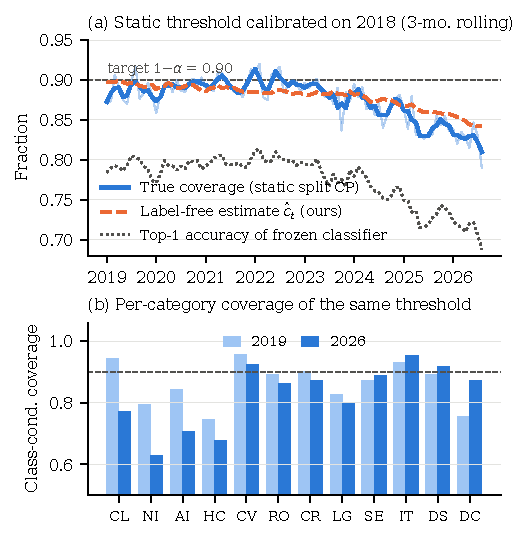
\includegraphics[width=\columnwidth]{fig1_expiry.pdf}
\caption{Deployment A. (a) A threshold calibrated on 2018 keeps $\approx$90\% coverage until 2022 and then erodes; the label-free estimate $\chat_t$ (dashed) follows it. (b) Erosion is concentrated in categories whose content changed most (CL, NI, AI, HC).}
\label{fig:expiry}
\end{figure}

\section{Results}\label{sec:results}
\subsection{Guarantees expire, and not because of label shift}\label{sec:expiry}
Fig.~\ref{fig:expiry}(a) shows the coverage of the static threshold. Yearly means are 0.887, 0.890, 0.894, 0.898 for 2019--2022, i.e.\ essentially nominal for four years, then 0.882, 0.872, 0.844 and 0.825 for 2023--2026. Top-1 accuracy of the frozen classifier falls in parallel from 0.79 to 0.71. The inflection coincides with the LLM-era reshaping of CS abstracts. Over the whole stream, 19.6\% of months fall below 0.85 (Table~\ref{tab:main}).

Two observations locate the cause. First, Mondrian calibration, which is immune to changes in category proportions by construction, gives the same mean coverage (0.874) and \emph{more} failing months (22.8\%): label shift is not the driver. Second, per-category coverage (Fig.~\ref{fig:expiry}(b)) drops from 0.94 to 0.77 for cs.CL, 0.80 to 0.63 for cs.NI and 0.84 to 0.71 for cs.AI, while cs.CV and cs.IT are unchanged. The loss is within-category content drift of the kind a single global or per-class quantile cannot absorb.

\subsection{The classifier knows its coverage is slipping}\label{sec:estimator}
The dashed curve in Fig.~\ref{fig:expiry}(a) is $\chat_t(q_0)$, computed without any label after 2018. Its yearly means (0.896 to 0.847) shadow the true values; monthly Pearson correlation is 0.815 and MAE 0.014 (Deployment B: 0.837 / 0.020; TF-IDF: 0.809 / 0.016). The estimate is slightly optimistic in the worst year (0.847 vs.\ 0.825), consistent with the classifier becoming somewhat over-confident on unfamiliar inputs, but it flags the erosion months before a labeled audit would.

\begin{table*}[t]
\caption{Monthly coverage statistics over the test stream at target $1-\alpha=0.90$. \emph{Labels} = fraction of stream months whose labels the method consumes. \emph{Fail} = fraction of months with coverage $<0.85$. \selftrig{} budgets are listed per deployment (A/B/C). Rows are grouped by label use: none, budgeted, and every month; bold marks the best Cov./Min/Fail within the first two groups. $^{*}$ACI additionally needs each label immediately after serving.}
\label{tab:main}
\centering\footnotesize
\setlength{\tabcolsep}{3.4pt}
\begin{tabular}{@{}l c cccc @{\hspace{6pt}} cccc @{\hspace{6pt}} cccc@{}}
\toprule
& & \multicolumn{4}{c}{A: MiniLM, cal.\ 2018 (92 mo.)} & \multicolumn{4}{c}{B: MiniLM, cal.\ 2021 (56 mo.)} & \multicolumn{4}{c}{C: TF-IDF, cal.\ 2018 (92 mo.)}\\
\cmidrule(lr){3-6}\cmidrule(lr){7-10}\cmidrule(lr){11-14}
Method & Labels & Cov. & Min & Fail & Size & Cov. & Min & Fail & Size & Cov. & Min & Fail & Size\\
\midrule
Static & 0 & 0.876 & 0.790 & 0.196 & 1.32 & 0.871 & 0.772 & 0.286 & 1.27 & 0.876 & 0.773 & 0.228 & 1.39\\
Mondrian (static) & 0 & 0.874 & 0.777 & 0.228 & 1.46 & 0.871 & 0.807 & 0.214 & 1.42 & 0.882 & 0.808 & 0.130 & 1.59\\
\selfcal{} (ours) & 0 & \textbf{0.898} & \textbf{0.850} & \textbf{0.000} & 1.44 & \textbf{0.885} & \textbf{0.825} & \textbf{0.054} & 1.34 & \textbf{0.911} & \textbf{0.858} & \textbf{0.000} & 1.65\\
\midrule
Periodic-6 & 0.17 & \textbf{0.895} & 0.845 & 0.022 & 1.43 & \textbf{0.896} & \textbf{0.833} & \textbf{0.036} & 1.41 & 0.895 & 0.857 & \textbf{0.000} & 1.53\\
Periodic-12 & 0.08 & 0.889 & 0.840 & 0.033 & 1.40 & 0.893 & 0.823 & \textbf{0.036} & 1.38 & 0.890 & 0.850 & \textbf{0.000} & 1.49\\
Random-0.1 & 0.10 & \textbf{0.895} & 0.840 & 0.024 & 1.44 & 0.890 & 0.831 & 0.059 & 1.37 & 0.896 & 0.837 & 0.023 & 1.54\\
\selftrig{} (ours) & .03/.04/.04 & 0.890 & \textbf{0.847} & \textbf{0.011} & 1.40 & 0.884 & 0.797 & 0.054 & 1.33 & \textbf{0.906} & \textbf{0.858} & \textbf{0.000} & 1.61\\
\midrule
Sliding-1 & 1.00 & 0.899 & 0.843 & 0.011 & 1.46 & 0.899 & 0.850 & 0.000 & 1.43 & 0.899 & 0.840 & 0.033 & 1.56\\
Sliding-12 & 1.00 & 0.896 & 0.847 & 0.011 & 1.43 & 0.893 & 0.838 & 0.018 & 1.39 & 0.896 & 0.857 & 0.000 & 1.52\\
Weighted $0.9^{\Delta t}$ & 1.00 & 0.895 & 0.847 & 0.022 & 1.43 & 0.891 & 0.830 & 0.018 & 1.37 & 0.895 & 0.852 & 0.000 & 1.51\\
ACI $\gamma{=}0.01$ & 1.00$^{*}$ & 0.900 & 0.885 & 0.000 & 1.49 & 0.900 & 0.890 & 0.000 & 1.46 & 0.900 & 0.890 & 0.000 & 1.59\\
\bottomrule
\end{tabular}
\end{table*}

\subsection{Label-free recalibration restores coverage}
Table~\ref{tab:main} and Fig.~\ref{fig:methods} compare all methods. In Deployment A, \selfcal{} lifts mean coverage from 0.876 to 0.898, raises the worst month from 0.790 to 0.850, and eliminates failing months entirely, using no label after 2018. This equals Sliding-1 (0.899, worst 0.843, 1.1\% failing), which relabels every month, and is within noise of Weighted CP. It does so by growing sets from 1.32 to 1.44 labels on average, the same price the labeled methods pay (1.43--1.46). ACI remains the strongest (0.900, worst 0.885) but requires the label of every single abstract immediately after it is served, which is the scenario our setting rules out.

Deployment B is harder: the classifier is trained on data up to 2020 and immediately meets the 2023+ shift. \selfcal{} still recovers half of the lost coverage (0.871 to 0.885, worst month 0.772 to 0.825) but trails the labeled window (0.899). The gap is explained by the estimator's optimism: its MAE is 0.020 here versus 0.014 in A. We consider this the honest boundary of the method---label-free monitoring is valuable, but it cannot fully substitute for labels when the model becomes markedly over-confident.

\begin{figure}[t]
\centering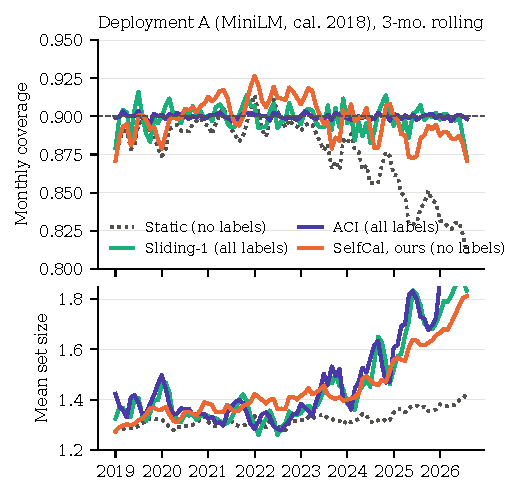
\includegraphics[width=\columnwidth]{fig2_methods.pdf}
\caption{Monthly coverage (top) and set size (bottom) for the static threshold, two label-rich baselines, and \selfcal{}. \selfcal{} keeps coverage near target and expands sets during the 2023--2026 drift, without labels.}
\label{fig:methods}
\end{figure}

\subsection{Spending labels only when needed}
Fig.~\ref{fig:budget} plots mean coverage deviation against label budget. In Deployment A, \selftrig{} fires three times (April 2022, January 2025, July 2026), a 3.3\% budget, and attains a deviation of 0.016, equal to Random-0.1 (10\% budget), within 0.001 of Periodic-6 (17\%), and better than Periodic-12 (8\%, 0.017). \selfcal{} at zero budget (0.014) sits on the frontier defined by fully-labeled Sliding-1 (0.014). In Deployment B, \selftrig{} (3.6\%) matches Periodic-12 (8.3\%) and Random-0.1 (10\%); more labels do still help there, with Random-0.5 reaching 0.017. The trigger months are interpretable: each follows a visible dip in Fig.~\ref{fig:expiry}(a).

\begin{figure}[t]
\centering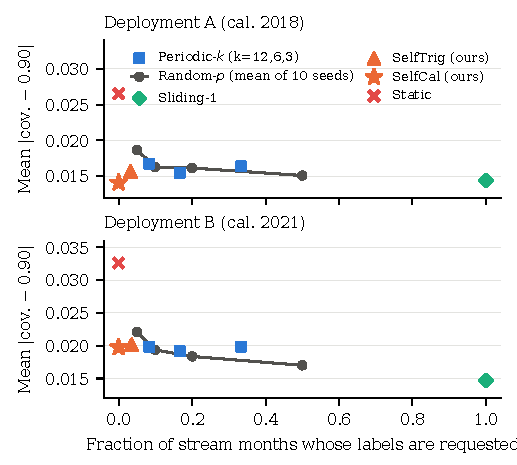
\includegraphics[width=\columnwidth]{fig3_budget.pdf}
\caption{Coverage deviation vs.\ label budget. \selfcal{} (zero labels) and \selftrig{} ($\le$4\% of months) reach the accuracy of methods that relabel 10--100\% of months.}
\label{fig:budget}
\end{figure}

\subsection{Robustness and an ablation}
\textbf{Lexical model.} With TF-IDF features the static guarantee erodes faster (0.887 to 0.818, worst month 0.773), as expected for a vocabulary-bound model. \selfcal{} and \selftrig{} both remove all failing months, with \selfcal{} slightly over-covering (0.911, sets 1.65).

\textbf{Temperature scaling matters.} Without temperature scaling the TF-IDF logistic regression is badly miscalibrated ($\delta{=}0.155$); \selfcal{} then over-covers at 0.922 with sets of 1.75, and \selftrig{} fires in 33\% of months. After scaling ($T{=}0.62$, $\delta{=}0.004$) both behave as in Table~\ref{tab:main}. For MiniLM the scaling is nearly neutral ($T{=}0.91$, $\delta{=}{-}0.005$). The magnitude of $\delta$ is thus a cheap, label-free-at-deployment diagnostic of whether the estimator can be trusted.

\textbf{Stricter target.} At $\alpha{=}0.05$ (Deployment A) the static threshold decays from 0.939 to 0.901 by 2026 and fails in 2.2\% of months; \selfcal{} holds 0.945 with worst month 0.900 and no failures, versus 0.949 for Sliding-1.

\section{Limitations and Conclusion}
Our estimator inherits the calibration of the base model, offers no distribution-free guarantee, and became optimistic by up to two points when the classifier was most stale; a formal bound relating $|\chat_t-\bar c_t|$ to calibration error under drift is an open question. We evaluated one stream, one score function, and linear heads on frozen features; deep fine-tuned classifiers may drift in confidence differently. Monthly batches of 600 are large, and smaller batches will make $\chat_t$ noisier.

Nevertheless, the picture is clear. On a natural, decade-long stream of 98k scientific abstracts, a conformal guarantee calibrated once quietly expired after about four years, and the expiry was caused by content drift that class-conditional calibration cannot fix. The frozen classifier's own temperature-scaled probabilities contain enough signal to detect the expiry and, in most cases, to repair it: \selfcal{} restored nominal coverage with no labels, and \selftrig{} did so while labeling roughly one month in thirty. For practitioners who wrap large-scale text classifiers in conformal sets, we recommend monitoring $\chat_t$ as routinely as accuracy, and treating a drop in it as the signal to recalibrate. All code, sampling scripts and result tables are available at \url{https://github.com/jeremiahdjoseph843-dot/conformal-expiry}.

\bibliographystyle{IEEEtran}
\bibliography{refs}
\end{document}
